\documentclass{article}
\usepackage{tikz}
\usetikzlibrary{automata, positioning, arrows.meta}
\usepackage{pdflscape}

\begin{document}
\begin{landscape}
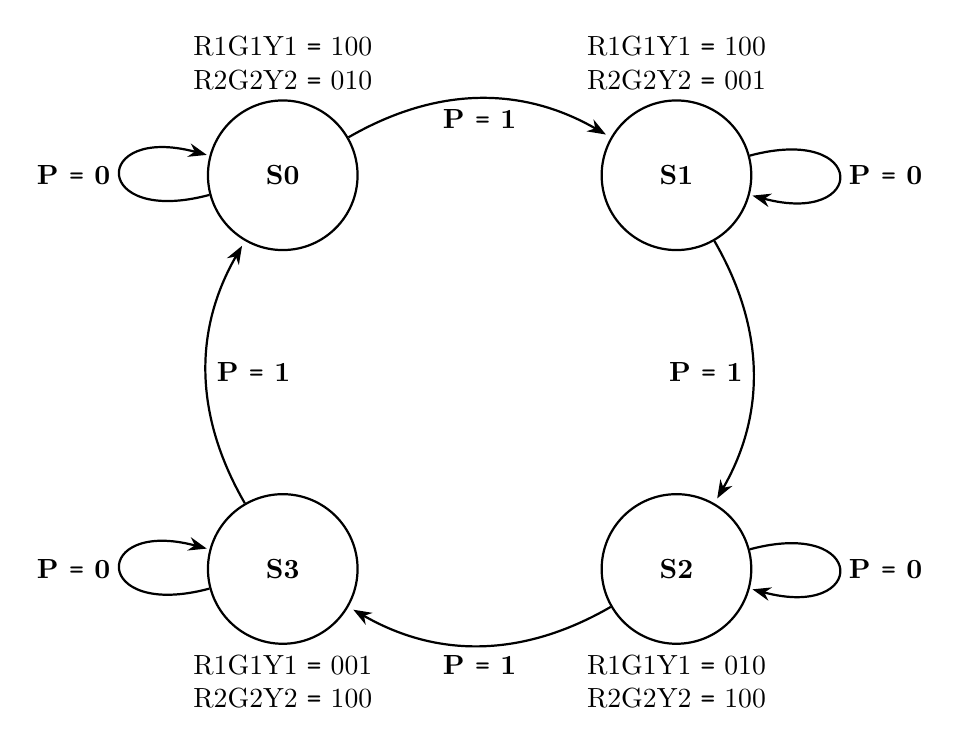
\begin{tikzpicture}[->,>=Stealth,shorten >=2pt,auto,node distance=5cm,thick]
  \tikzstyle{every state}=[fill=white,draw=black,text=black]

  \node[state, minimum width=1.9cm, minimum height=1.9cm] (S0) {\textbf{S0}};
  \node[state, minimum width=1.9cm, minimum height=1.9cm] (S1) [right of=S0] {\textbf{S1}};
  \node[state, minimum width=1.9cm, minimum height=1.9cm] (S2) [below of=S1] {\textbf{S2}};
  \node[state, minimum width=1.9cm, minimum height=1.9cm] (S3) [left of=S2] {\textbf{S3}};

  \path (S0) edge [bend left] node[midway, below][font=\bfseries] {P \texttt{=} 1} (S1)
        (S1) edge [bend left] node[midway, left][font=\bfseries] {P \texttt{=} 1} (S2)
        (S0) edge [loop left] node[midway, left][font=\bfseries] {P \texttt{=} 0} (S0)
        (S1) edge [loop right] node[midway, right][font=\bfseries] {P \texttt{=} 0} (S1)
        (S2) edge [bend left] node[midway, below][font=\bfseries] {P \texttt{=} 1} (S3)
        (S3) edge [bend left] node[midway, right][font=\bfseries] {P \texttt{=} 1} (S0)
        (S2) edge [loop right] node[midway, right][font=\bfseries] {P \texttt{=} 0} (S2)
        (S3) edge [loop left] node[midway, left][font=\bfseries] {P \texttt{=} 0} (S3);
        
  \node[align=center, text width=5cm, above] at (S0.north) {R1G1Y1 \texttt{=} 100\\R2G2Y2 \texttt{=} 010};
  \node[align=center, text width=5cm,above] at (S1.north) {R1G1Y1 \texttt{=} 100\\R2G2Y2 \texttt{=} 001};
  \node[align=center, text width=5cm,below] at (S2.south) {R1G1Y1 \texttt{=} 010\\R2G2Y2 \texttt{=} 100};
  \node[align=center, text width=5cm,below] at (S3.south) {R1G1Y1 \texttt{=} 001\\R2G2Y2 \texttt{=} 100};
  
\end{tikzpicture}
\end{landscape}
\end{document}